% ================================================================
\section{Introduction}\label{sec:intro}

Model-predictive control (MPC) is a powerful framework for controlling
highly dynamic robots subject to state and input constraints~\cite{tinympc}.
TinyMPC~\cite{tinympc} demonstrated that, by caching the
infinite-horizon discrete algebraic Riccati equation (DARE) solution
offline and performing only matrix--vector products online,
the ADMM-based MPC solver can run on microcontrollers with as little
as 192\,kB of RAM at rates exceeding 500\,Hz.

A key assumption in TinyMPC is that the dynamics are linearized
at a \emph{fixed operating point}---typically the hover equilibrium
for a quadrotor.
This is reasonable for near-hover regulation but becomes a limitation
for aggressive trajectory tracking, where the true linearization
varies significantly along the reference.
The standard remedy---online relinearization at each timestep---requires
Jacobian evaluation (via automatic differentiation or finite differences)
and a fresh DARE solve, both of which are computationally expensive
and ill-suited for resource-constrained platforms.

We observe that quadrotor dynamics are \emph{differentially flat}
with flat output $\by = (p_x, p_y, p_z, \psi)$~\cite{mellinger2011,murray1995}.
This classical property has been widely used for trajectory
generation~\cite{mellinger2011,mueller2015}, but its implications
for \emph{MPC solver structure} have received less attention.
We show that flatness enables a closed-form parameterization of
both the equilibrium and the Jacobian by a single four-dimensional
\emph{flat parameter}
$\balpha = (a_x, a_y, a_z, \psi) \in \R^4$,
representing the commanded translational acceleration and yaw angle.
Because the resulting expressions involve only elementary trigonometric
and algebraic operations, they require no automatic differentiation
and are directly implementable on FPGAs.

Crucially, because $\balpha$ is four-dimensional---compared to the
$n=12$ dimensional state---it serves as a natural
\emph{scheduling variable} for the DARE solution.
This connects our approach to classical gain scheduling~\cite{rugh2000}
and linear parameter-varying (LPV) control~\cite{shamma1991},
but with the scheduling space compressed from $\R^n$ to $\R^4$
by the flat map.
We make this connection precise in Section~\ref{sec:analytic}
and show that the Analytic Template is equivalent to
a first-order gain schedule over $\balpha$, where the gain
sensitivity is obtained from perturbation analysis of the
DARE~\cite{hewer1971,konstantinov1993}.

Building on this observation, we propose three extensions of TinyMPC:

\begin{enumerate}
  \item \textbf{Flat Template MPC} (Section~\ref{sec:flat_template}):
    Precompute DARE caches at a grid of $\balpha$ values offline.
    Online, look up the nearest cache and run $K_{\mathrm{ADMM}}$
    ADMM iterations as in standard TinyMPC, but with
    $\balpha$-specific
    matrices $(A_d, B_d, K_\infty, P_\infty, C_1, C_2)$.
  \item \textbf{Analytic Template} (Section~\ref{sec:analytic}):
    Precompute the gain $K_0$ at hover and its four partial
    derivatives $\partial K / \partial \alpha_i$ offline.
    Online, interpolate $K(\balpha) \approx K_0 + \sum_i \delta\alpha_i \, \partial_i K$
    and apply a single feedback step---no ADMM iterations, no constraint
    projection.
    The total cost is ${\sim}260$ multiply-accumulate (MAC) operations.
  \item \textbf{Barrier-Augmented Template} (Section~\ref{sec:barrier}):
    Absorb log-barrier constraint penalties into the DARE cache,
    so that the zero-iteration controller inherently avoids
    actuator limits.
    Optional Newton--IPM refinement online yields hard constraint
    satisfaction at quadratic convergence.
\end{enumerate}

All flat-parameterized variants shift the coordinate frame to
the flat equilibrium $(x^*(\balpha), u^*(\balpha))$,
so the solver always operates in a neighborhood of zero
error---regardless of the trajectory aggressiveness.
Fig.~\ref{fig:hierarchy} illustrates the pipeline.

\begin{figure}[t]
  \centering
  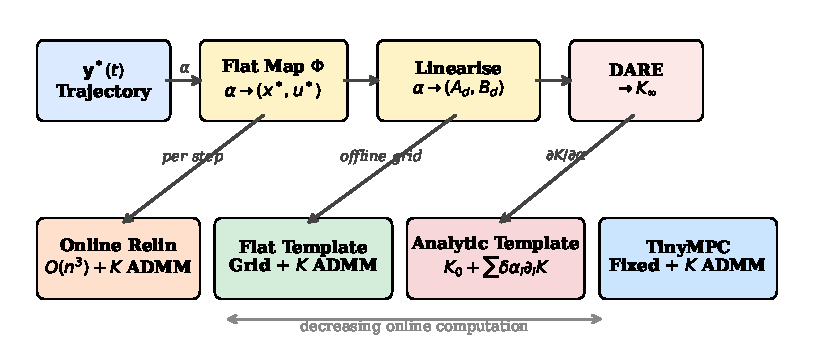
\includegraphics[width=\columnwidth]{figures/fig_hierarchy.pdf}
  \caption{Controller hierarchy.
    The flat map $\Phi$ and analytic linearization (yellow) are shared
    by all flat-parameterized variants.
    Moving right trades online computation for approximation:
    Online Relinearization re-solves DARE per step;
    Flat Template looks up a precomputed cache;
    the Analytic Template interpolates $K(\balpha)$ in ${\sim}260$ ops.}
  \label{fig:hierarchy}
\end{figure}

\subsection*{Contributions}
\begin{itemize}
  \item An explicit, autograd-free linearization of quadrotor
    dynamics parameterized by $\balpha \in \R^4$
    (Section~\ref{sec:linearize}).
  \item Flat Template MPC: an $\balpha$-indexed cache family for
    TinyMPC's ADMM solver (Section~\ref{sec:flat_template}).
  \item Analytic Template: a zero-iteration controller with
    first-order gain approximation (Section~\ref{sec:analytic}).
  \item Barrier-Augmented Template: absorbing log-barrier constraint
    information into the DARE cache for zero-iteration
    constraint-aware control, with optional IPM refinement
    at quadratic convergence (Section~\ref{sec:barrier}).
  \item Convergence analysis: quadratic gain approximation error
    from flatness-compressed scheduling, and exponential
    time-contraction with explicit rate--conservatism tradeoff
    (Section~\ref{sec:convergence}).
  \item Preliminary numerical validation comparing four controller
    variants on hover, figure-eight, and constrained circle tracking
    (Section~\ref{sec:experiments}).
\end{itemize}
